\documentclass{article}
\usepackage[top=1in, bottom=1in, left=1in, right=1in]{geometry}
\usepackage{polski}
\usepackage[utf8]{inputenc}
\usepackage{graphicx}
\begin{document}
\title{\huge\bfseries Sprawdzanie prawa Malusa}
\date{}
\author{}
\maketitle
\section{Wstęp teoretyczny}
\subsection{Fala elektromagnetyczna}
Fala elektromagnetyczna to połączenie pola elektrycznego i magnetycznego. Pole elektromagnetyczne może się rozchodzić w przestrzeni z prędkością światła. Fala elektromagnetyczna to rozchodzące się w przestrzeni sprężone pole elektryczne. Wielkością charakteryzującą fale jest częstotliwość.
\subsection{Polaryzacja fali}
Polaryzacja to własność fali poprzecznej(np. światła). Fala spolaryzowana oscyluje(drga) tylko w wybranym kierunku. Dla fali mechanicznej jest to kierunek przesunięć\\\\
Polaryzacja fali elektromagnetycznej to kierunek wzajemnie prostopadłych pól: elektrycznego i magnetycznego\\\\
Polaryzacja liniowa drganie odbywa się wzdłuż linii prostej. Każde drganie można przedstawić jako sumę drgań wzdłóż osi $X$ i $Y$.\\
Polaryzacja kołowa drganie to odpowiada ruchowi po okręgu. Można je rozłożyć na dwa drgania o jednakowych amplitudach, ale o fazach dokładnie przesuniętych o $90^{\circ}C$ lub $270^{\circ}C$.
\subsection{Prawo Malusa}
Prawo Malusa określa natężenie światła spolaryzowanego po przejściu przez polaryzator w zależności od kąta ustawienia analizatora względem polaryzatora.
$$I = I_0 * \cos^2\alpha$$

\begin{center}
$I_0$ - natężenie światła padającego \\
$\alpha$ - kąt między płaszczyzną polaryzacji światła padającego i płaszczyzną polaryzacji polaryzatora
\end{center}

\section{Przebieg i cel ćwiczenia}
Celem naszego ćwiczenia było sprawdzenie prawa Malusa, poprzez obracanie analizatorem o $5^{\circ}$. Wyniki zapisywaliśmy z miliamperomierza. Obrót analizatora o $90^{\circ}$ względem polaryzatora spowoduje wygaszenie wiązki.

\subsection{Opracowanie pomiarów}
Obracaliśmy analizatorem o $5^{\circ}$ zaczynając od $0^{\circ}$, a kończąc na $360^{\circ}$. Wyniki zapisywaliśmy z miliamperomierza firmy METEX, model $M-3650D$. Dokładność amperomierza wynosi $+-1\%$ dla $+- 3$ cyfr.

\begin{center}
    \begin{tabular}{|c|c|c|c|c|c|c|c|}
    \hline
    $\phi , ^{\circ} $ & $i , mA$ & $\phi , ^{\circ}$ & $i , mA$ & $\phi , ^{\circ}$ & $i , mA$ & $\phi , ^{\circ}$ & $i , mA$\\ \hline
    $0$ & $0,0007$ & $95$ & $0,0125$ & $185$ & $0,0004$ & $275$ & $0,0117$\\ \hline
    $5$ & $0,0004$ & $100$ & $0,0130$ & $190$ & $0,0001$ & $280$ & $0,0120$\\ \hline
    $10$ & $0,0002$ & $105$ & $0,0133$ & $195$ & $0,0001$ & $285$ & $0,0120$\\ \hline
    $15$ & $0,0001$ & $110$ & $0,0133$ & $200$ & $0,0001$ & $290$ & $0,0120$\\ \hline
    $20$ & $0,0001$ & $115$ & $0,0131$ & $205$ & $0,0002$ & $295$ & $0,0119$\\ \hline
    $25$ & $0,0001$ & $120$ & $0,0126$ & $210$ & $0,0004$ & $300$ & $0,0115$\\ \hline
    $30$ & $0,0002$ & $125$ & $0,0120$ & $215$ & $0,0007$ & $305$ & $0,0109$\\ \hline
    $35$ & $0,0004$ & $130$ & $0,0112$ & $220$ & $0,0014$ & $310$ & $0,0101$\\ \hline
    $40$ & $0,0007$ & $135$ & $0,0102$ & $225$ & $0,0022$ & $315$ & $0,0092$\\ \hline
    $45$ & $0,0014$ & $140$ & $0,0089$ & $230$ & $0,0031$ & $320$ & $0,0082$\\ \hline
    $50$ & $0,0023$ & $145$ & $0,0077$ & $235$ & $0,0041$ & $325$ & $0,0071$\\ \hline
    $55$ & $0,0033$ & $150$ & $0,0064$ & $240$ & $0,0052$ & $330$ & $0,0059$\\ \hline
    $60$ & $0,0044$ & $155$ & $0,0052$ & $245$ & $0,0064$ & $335$ & $0,0048$\\ \hline
    $65$ & $0,0056$ & $160$ & $0,0040$ & $250$ & $0,0075$ & $340$ & $0,0037$\\ \hline
    $70$ & $0,0071$ & $165$ & $0,0028$ & $255$ & $0,0085$ & $345$ & $0,0027$\\ \hline
    $75$ & $0,0084$ & $170$ & $0,0020$ & $260$ & $0,0095$ & $350$ & $0,0019$\\ \hline
    $80$ & $0,0096$ & $175$ & $0,0014$ & $265$ & $0,0104$ & $355$ & $0,0012$\\ \hline
    $85$ & $0,0108$ & $180$ & $0,0007$ & $270$ & $0,0112$ & $360$ & $0,0007$\\ \hline
    $90$ & $0,0118$ &       &          &       &          &       &         \\ \hline
    \end{tabular}
\end{center}
$$$$\\
\section{Opracowanie wyników pomiarów}
Sporządziliśmy wykres zależnośći wskazań miernika od kąta skręcenia analizatora względem polaryzatora\\\\\\\\\\\\\\\\\\\\\\\\\\\\\\\\\\\\\\\\\\\\\\\\\\\\\\\\\\\\
\begin{figure}
\centering
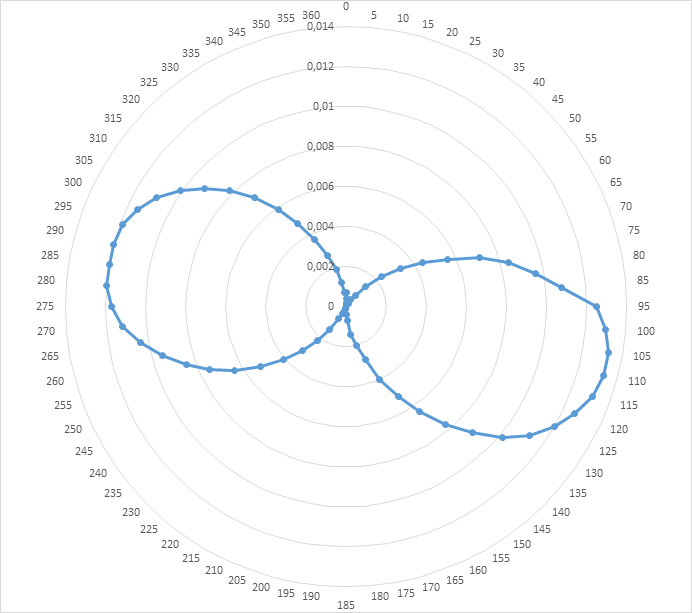
\includegraphics[width=18cm]{wykres2.png}
\end{figure}

Obliczyliśmy według prawa Malusa teoretyczne wartości prądu płynącego przez fotoopornik:
$$i_T = i_{max} \cdot \cos^2(\phi)$$
\begin{center} $i_{max} $ - maksymalne wskazanie amperomierza \end{center}
Amperomierz wskazywał maksymalną wartość równą $0,0133$ dla $105^{\circ}$ i  $110^{\circ}$. \\\\
Przykład obliczenia dla kąta $0^{\circ}$
$$i_T = 0,0133 \cdot cos^2(0^{\circ}) = 0,0133 $$
Wyniki zapisaliśmy do tabeli z dokładnością do czterech miejsc po przecinku:
\begin{center}
    \begin{tabular}{|c|c|c|c|c|c|c|c|}
    \hline
    $\phi , ^{\circ} $ & $i_T$ & $\phi , ^{\circ}$ & $i_T$ & $\phi , ^{\circ}$ & $i_T$ & $\phi , ^{\circ}$ & $i_T$\\ \hline
    $0$ & $0,0133$ & $95$ & $0,0001$ & $185$ & $0,0131$ & $275$ & $0,0001$\\ \hline
    $5$ & $0,0131$ & $100$ & $0,0004$ & $190$ & $0,0128$ & $280$ & $0,0004$\\ \hline
    $10$ & $0,0128$ & $105$ & $0,0008$ & $195$ & $0,0124$ & $285$ & $0,0008$\\ \hline
    $15$ & $0,0124$ & $110$ & $0,0015$ & $200$ & $0,0117$ & $290$ & $0,0015$\\ \hline
    $20$ & $0,0117$ & $115$ & $0,0023$ & $205$ & $0,0109$ & $295$ & $0,0023$\\ \hline
    $25$ & $0,0109$ & $120$ & $0,0033$ & $210$ & $0,0099$ & $300$ & $0,0033$\\ \hline
    $30$ & $0,0099$ & $125$ & $0,0043$ & $215$ & $0,0089$ & $305$ & $0,0043$\\ \hline
    $35$ & $0,0089$ & $130$ & $0,0054$ & $220$ & $0,0078$ & $310$ & $0,0054$\\ \hline
    $40$ & $0,0078$ & $135$ & $0,0066$ & $225$ & $0,0065$ & $315$ & $0,0066$\\ \hline
    $45$ & $0,0065$ & $140$ & $0,0078$ & $230$ & $0,0054$ & $320$ & $0,0078$\\ \hline
    $50$ & $0,0054$ & $145$ & $0,0089$ & $235$ & $0,0043$ & $325$ & $0,0089$\\ \hline
    $55$ & $0,0043$ & $150$ & $0,0099$ & $240$ & $0,0033$ & $330$ & $0,0099$\\ \hline
    $60$ & $0,0033$ & $155$ & $0,0109$ & $245$ & $0,0023$ & $335$ & $0,0109$\\ \hline
    $65$ & $0,0023$ & $160$ & $0,0117$ & $250$ & $0,0015$ & $340$ & $0,0117$\\ \hline
    $70$ & $0,0015$ & $165$ & $0,0124$ & $255$ & $0,0008$ & $345$ & $0,0124$\\ \hline
    $75$ & $0,0008$ & $170$ & $0,0128$ & $260$ & $0,0004$ & $350$ & $0,0128$\\ \hline
    $80$ & $0,0004$ & $175$ & $0,0131$ & $265$ & $0,0001$ & $355$ & $0,0131$\\ \hline
    $85$ & $0,0001$ & $180$ & $0,0133$ & $270$ & $0,0000$ & $360$ & $0,0133$\\ \hline
    $90$ & $0,0000$ &       &          &       &          &       &         \\ \hline
    \end{tabular}
\end{center}

$$$$\\
Na wykres radarowy nanieśliśmy wartości teoretyczne $i_T$\newpage

\begin{figure}
\centering
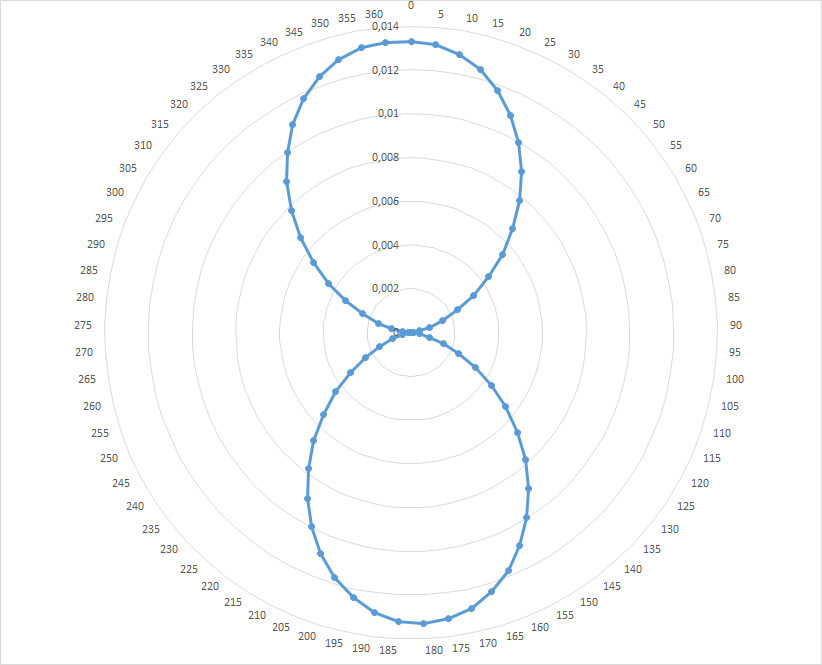
\includegraphics[width=18cm]{wykres1.png}
\end{figure}

Wykresy względem siebie są obrócone. Znaleźliśmy błąd zera, czyli określiliśmy o jaki kąt $\alpha$ należy obrócić wykres pomiarowy, by oba wykresy pasowały do siebie. Korzystając ze wzoru:
$$\alpha + \phi = \phi_T$$

Obliczyliśmy błąd zera dla wartości $0,0131$:

$$\alpha = \phi_T - \phi$$
$$\alpha = 5^{\circ} - 115^{\circ}$$
$$\alpha = -110^{\circ}$$

Błąd zera wynosi $-110^{\circ}$\\\\

Następnie sporządziliśmy skorygowany wykres radarowy $i = f(phi_T)$ 

\begin{figure}
\centering
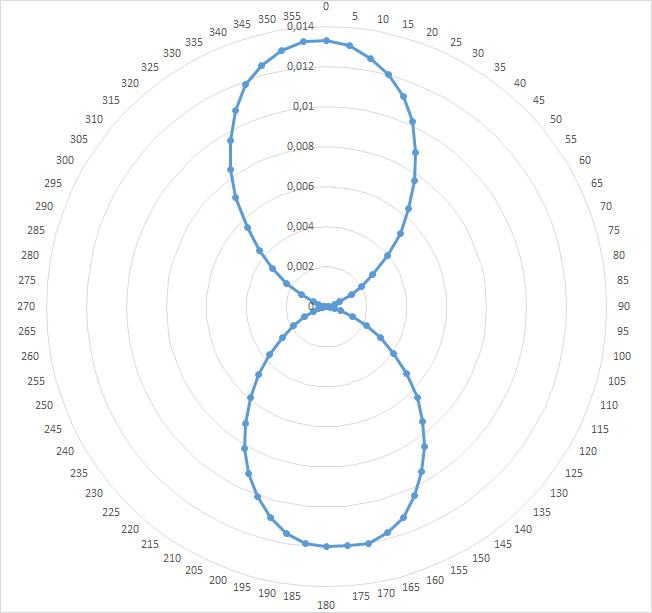
\includegraphics[width=18cm]{wykres3.png}
\end{figure}

$$$$ \newpage
Sporządziliśmy wykres zależności wskazań amperomierza $i(\phi_T) = i_{max} \cdot \cos^2(\phi_T)$. Na wykresie umieściliśmy prostą teoretyczną i prostą dopasowaną do punktów pomiarowych.

\begin{figure}
\centering
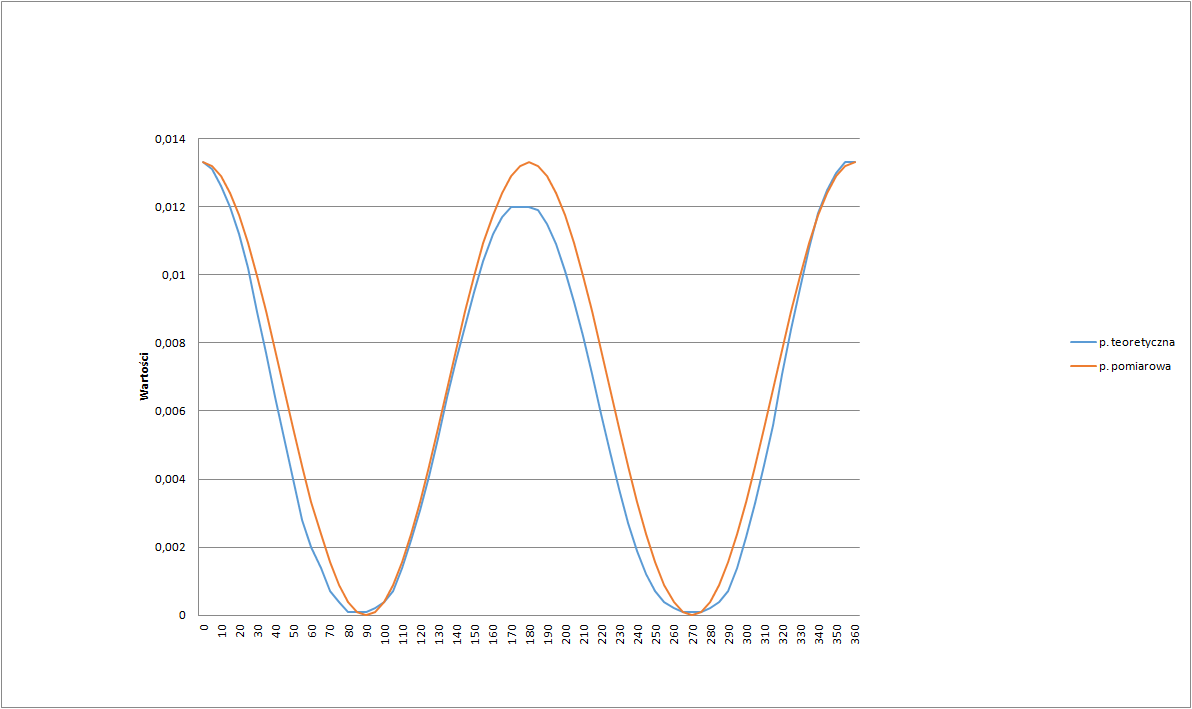
\includegraphics[width=18cm]{wykres4.png}
\end{figure}

\subsection{Wniosek}
Prawo Malusa zostało spełnione, ponieważ zmierzone natężenie było liniowo zależne od kwadratu cosinusa kąta położenia analizatora względem polaryzatora. Wyniki nie są dokładne ponieważ żarówka nie była stale przytwierdzona, przez co każdy ruch stanowiskiem badawczym powodował jej minimalne zmienianie położenia. 

\begin{flushright}
\begin{scriptsize}
Źródła: \textit{https://pl.wikibooks.org/wiki/Fale/Polaryzacja$\_$liniowa,$\_$ko$\%$C5$\%$82owa,$\_$eliptyczna$\_$fal} \\
\textit{http://www.szkolnictwo.pl/szukaj,Prawo$\_$Malusa}\\
\textit{http://fizyka.net.pl/ciekawostki/ciekawostki$\_$wn3.html}
\end{scriptsize}
\end{flushright}


\end{document}